\documentclass[]{article}
\usepackage{graphicx}
\usepackage{amssymb}
\usepackage{float}
\usepackage{float}
\usepackage{graphicx}% Include figure files
\usepackage{dcolumn}% Align table columns on decimal point
\usepackage{bm}% bold math

\usepackage{longtable}
\usepackage{multirow}

\bibliographystyle{unsrt}


\title{Using \textit{Maelstrom} to obtain orbital information about KIC 8264492 }
\author{Dillon Hanlon}
\date{\today}

\begin{document}


\maketitle
\begin{abstract}
    Binary and multi star systems have been crucial to our understanding of stellar structure and evolution due to the fact it can provide accurate measurement of stellar masses.
    This project focuses on using a third-party python software namely \textit{Maelstrom} to model the light curve and produce theoretical light curve data which gives information about the orbit of the binary star. 
    The result model showed a very high correlation with the original light curve data. The optimization parameters obtained were used to produce a simplistic plot of the orbital path of this binary star. 
\end{abstract}
\section{Introduction}
People think of stars as this lonely object in space that provide light, but many stars that are in space are actually in a binary system.
In fact, binary and even multiple system stars are much more common than single stars by at least a factor of 2:1 \cite{guszejnov2017protostellar}.
Components of binary systems either one or both components can pulsate, meaning that their brightness changes as a function of time. Typically the type of stars that appear in these systems are type A to type F main sequence stars \cite{garg2010high}.
Stars that pulsate can provide researchers with a clock also known as a standard candle to help aid their observations \cite{murphy2018finding}. 

Light curves are very useful to observe how the intensity (brightness) of a star changes as a function of time.
The shape of a light curve can give valuable information about the underlying physical processes producing the changes in the brightness (flux). 
As well, the shape of a light curve can indicate the relative sizes  and relative surface brightness of a pulsating stars \cite{russell1912determination}. Although light curves provide a great amount of detail, most work in astronomy has many contributions from many different experiments. Thus in order to get the full details of an stellar object data from many research experiments is required.

\section{Method}
This project focused on using \textit{Maelstrom}, an open source python package that models and analyzes binary light curves with a pulsating component in an attempt to model the light curve and produce information attributed to its orbital parameters. 
For this project the celestial object in study is the KIC 8264492, a binary star system with a $\delta$ Sct star component located in the open cluster field NGC 6866, located approximately 3900 light years away, and a mass of 1.87 $M_{\odot}$ and a temperature of $T_{eff} = 7992$K \cite{balona2013pulsation,shibahashi2015fm}.

\begin{figure}[H]
    \centering
    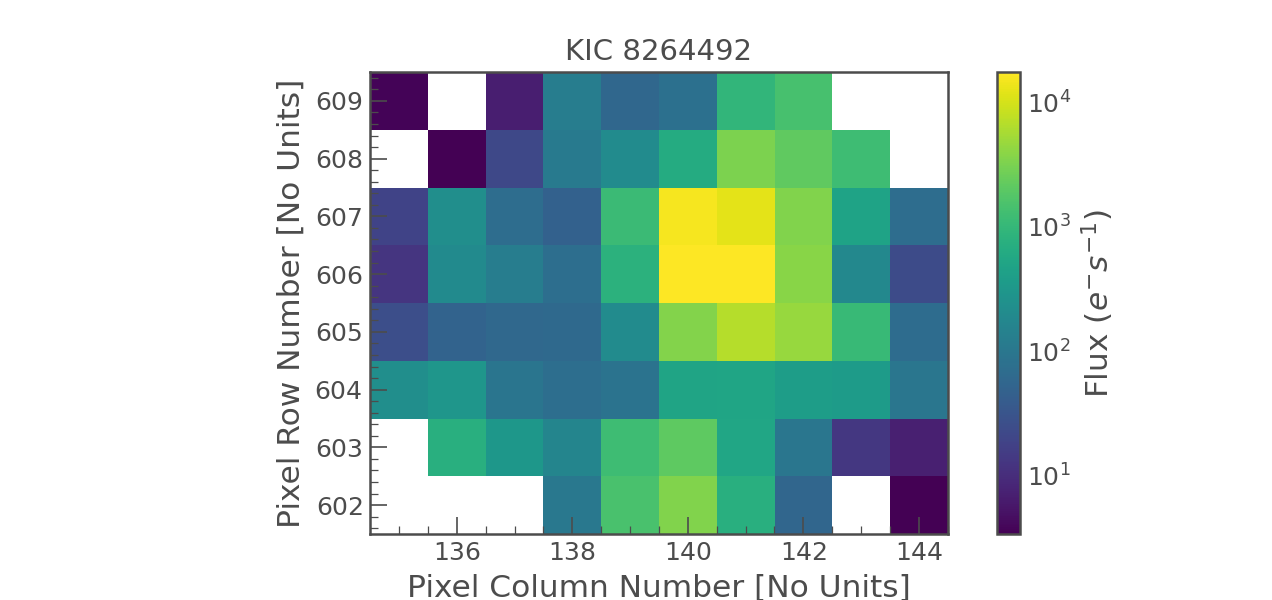
\includegraphics[width=1\linewidth]{Recover_Binary.png}
    \caption{Pixel image of the binary star KIC 8264492 extracted from keplers public data using the python module \textit{lightkurve}. Colorbar shows the brightness of the each pixel in $electrons / second$.}
    \label{fig:Recover_Binary}
\end{figure}


A third party python module, namely  \textit{lightkurve} was used initially to extrac the light curve data from a public database as well get a pixel image of the pulsating star indicating the brightness of that star. 
As can be seen from Fig \ref{fig:Recover_Binary} there is an intense region near the center of this image with flux on the order of $\sim$ 10$^4 electrons/second$ which representing the stars brightness at some time. 
\textit{Maelstrom} will use forward model algorithm on the light curve and attempt to optimize its orbital parameters, what \textit{Maelstrom} is doing is fitting the phase variation ($\tau$) at each point in the light curve which can be described by,

\begin{equation}
    y(t) = \sum_{j = 1}^{J} [A_j \cos(\omega_j (t - \tau)) + B_j \sin(\omega_j (t - \tau) ] + \epsilon
\label{eq:PhaseVariation}    
\end{equation}
where $A_j$ and $B_j$ define the mode ampitudes, $\omega$ is the angular frequency and $\epsilon$ describes variation unaccounted for by our pulsation mode
This equation describes the time-dependent flux variations due to $J$ pulsation modes and therefore must also include a time-delay term $\tau$ \cite{hey2020forward}.
\noindent
The light curve for the binary star used in this project can be seen in Fig \ref{fig:Lightcurve}.
The module \textit{lightkurve} subtracts 2454844 days which is the Kepler zero time from the time data. 
Therefore all times are reported in a Barycentric Kepler Julian Date (BKJD), doing this corrects for differences in the earths position with respect to the center of the solar system \cite{Eastman_2010}. 

\begin{figure}[H]
    \centering
    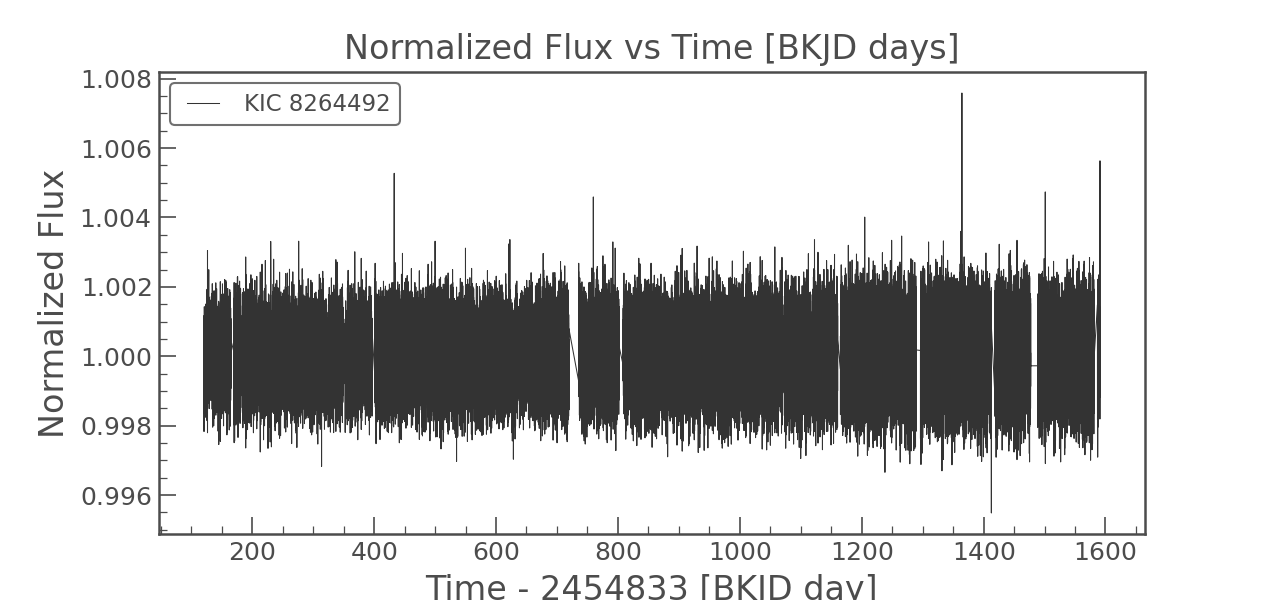
\includegraphics[width=1\linewidth]{Lightcurve.png}
    \caption{Normalized flux vs time reported in Barycentric Kepler Julian Date (BKJD) for KIC KIC 8264492.}
    \label{fig:Lightcurve}
\end{figure}


\section{Results}
After the light curve has been passed into \textit{Maelstroms} a forward modelling algorithm begins. 
Fig \ref{fig:timedelay} shows the extracted time delay values from the original light curve (black points) with the theoretical results obtained from the optimized parameters (blue curve).

\begin{figure}[H]
    \centering
    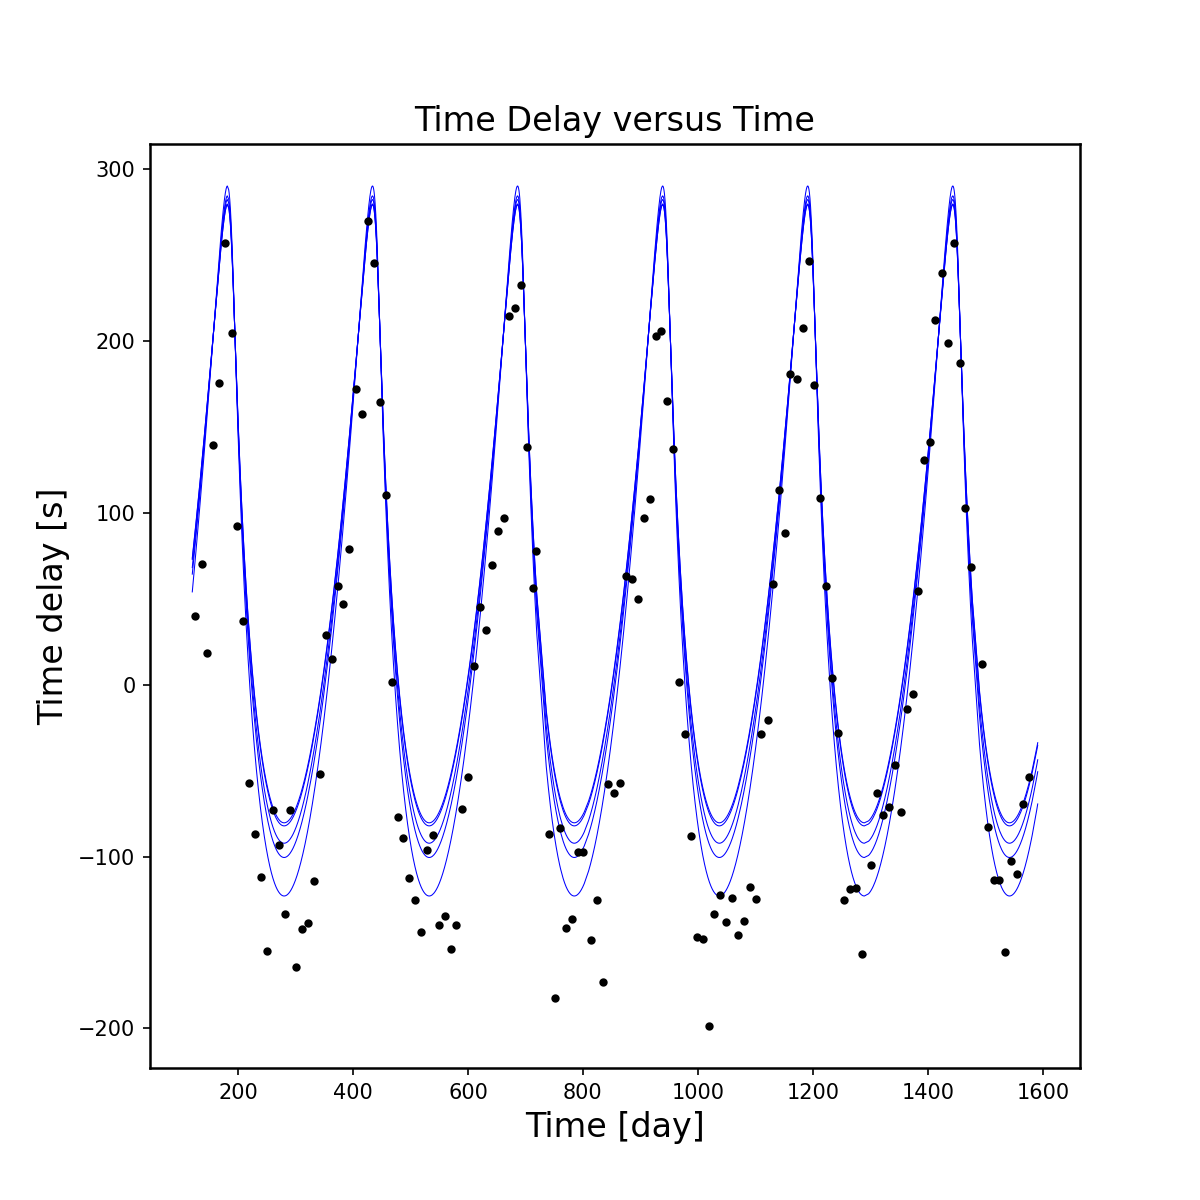
\includegraphics[width=1\linewidth]{time_delay.png}
    \caption{Time delay as a function of time for both the original data extracted from the original light curve (black dot) and the theoretical fit (blue curve).}
    \label{fig:timedelay}
\end{figure}
This essentially is showing how the distance the star is travelling in orbit influences how long it takes for the signal to be achieved, since the distance between the star and observer is changing. It is possible then to extract the optimized orbital parameters from Fig \ref{fig:timedelay} which are presented in Table \ref{tab: OptParam}.
\begin{table*}[htp] 
\centering
% \footnotesize\setlength{\tabcolsep}{3.5pt}
\caption{Table of optimized orbital parameters extracted from time delay signal as shown in Fig \ref{fig:timedelay}.}
\setlength{\extrarowheight}{2pt}
\begin{tabular}{c | c}
Orbital Parameter & Value [Unit]\\
\hline
    Period  & 2  \\
    Semi-Major Axis & 4\\
    Eccentricity & 6\\
    Orbital Period & \\
    Oscillation Modes & \\
\end{tabular} 
\label{tab: OptParam}
\end{table*}

\noindent
From these parameters it is possible to make an estimate of the shape of the elliptical orbit for this star. Knowing that the semi-minor axis is related to the semi-major axis by a factor of $1/2$, then it is possible to make a simplistic model of the orbit as shown in Fig \ref{fig:Orbit}.

\begin{figure}[H]
    \centering
    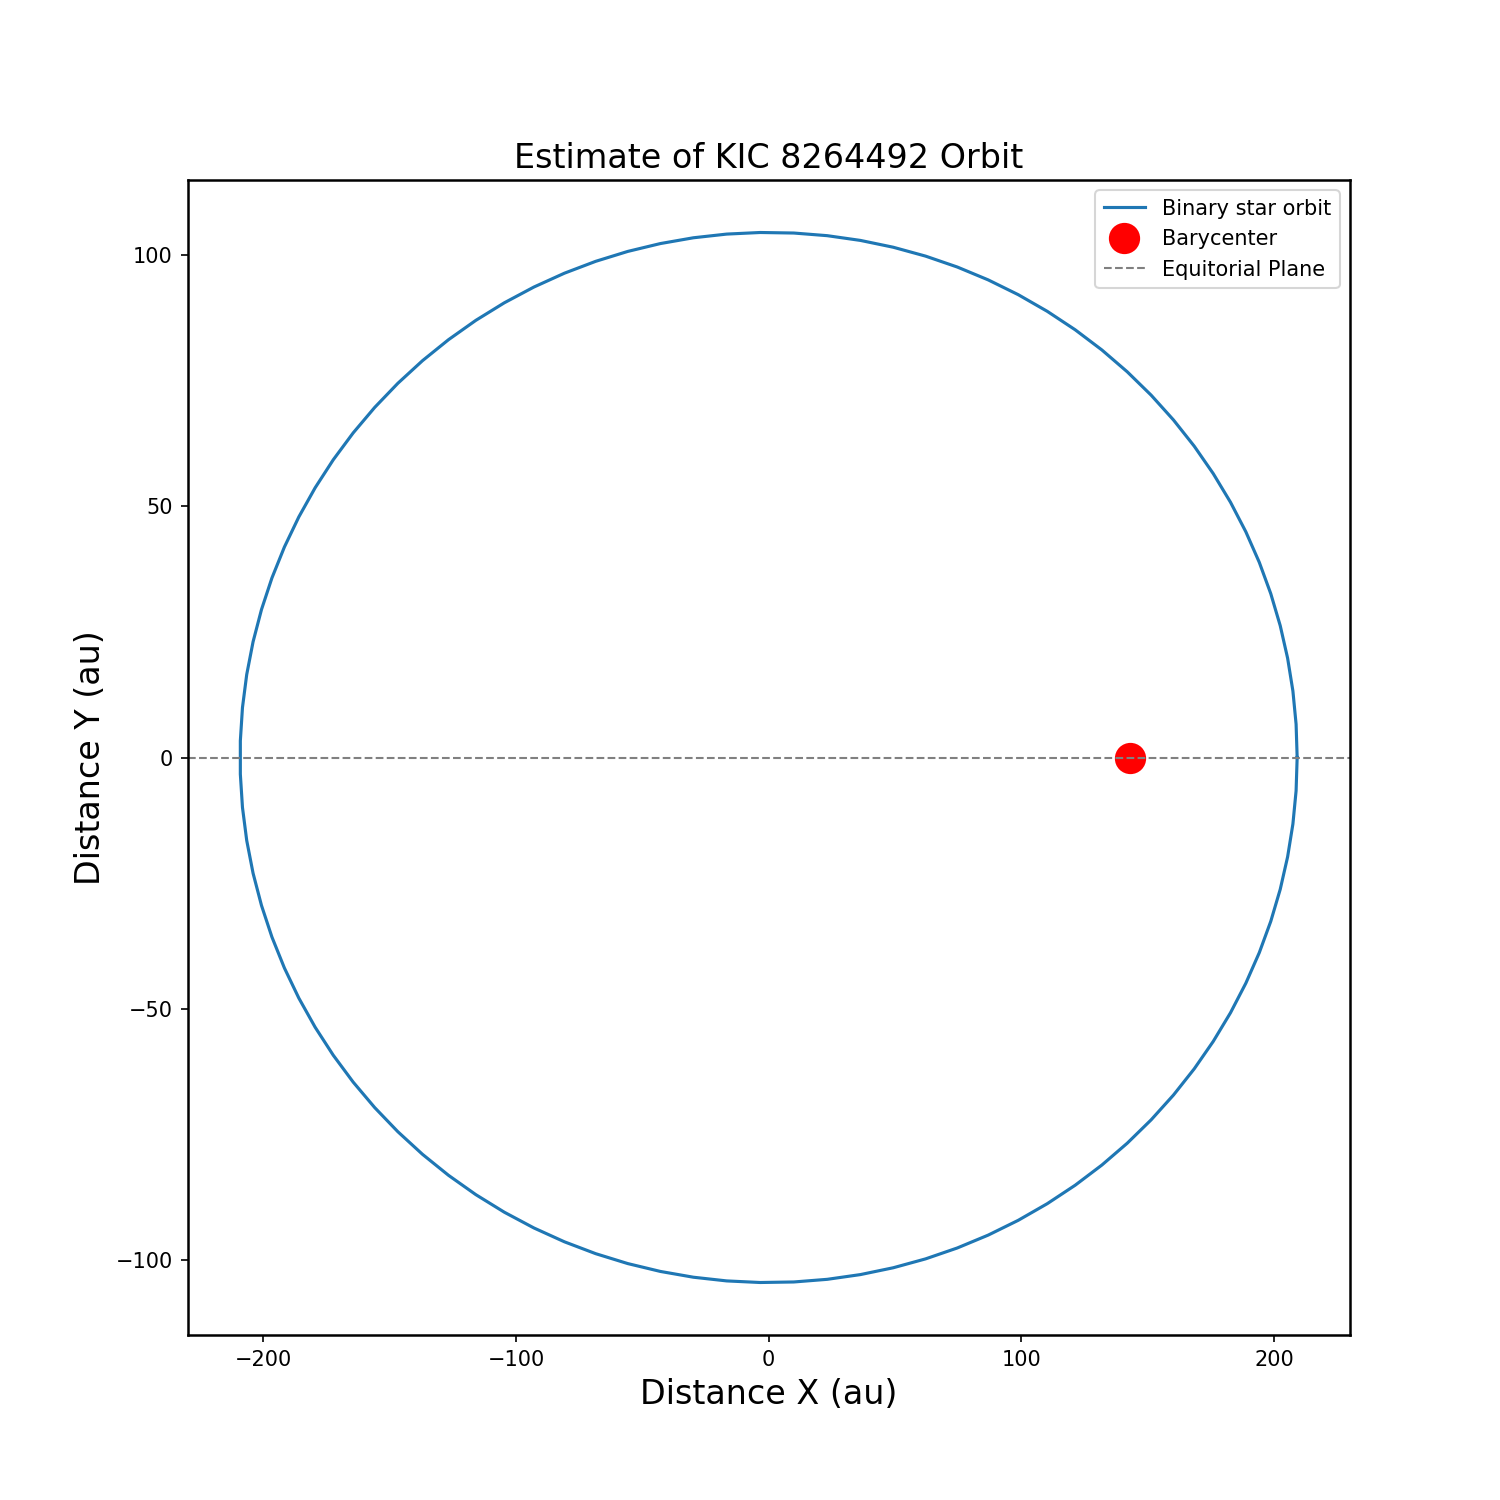
\includegraphics[width=1\linewidth]{orbit.png}
    \caption{Simplistic orbital ellipse derived from the optimized orbital parameters obtained via forward modelling. Red circle represents an estimate of the barycenter for the binary system.}
    \label{fig:Orbit}
\end{figure}
\noindent
Also in this figure is an estimate of where the center of mass (barycenter) for the two stars would be.
Since the orbital parameters of the other star in binary is unknown, it is not possible to make a schematic of that orbit.

The \textit{Maelstrom} package also makes it possible to extract the theoretical light curve from the time delay signal which is shown in Fig \ref{fig:LightcurveOptimized}.
\begin{figure}[H]
    \centering
    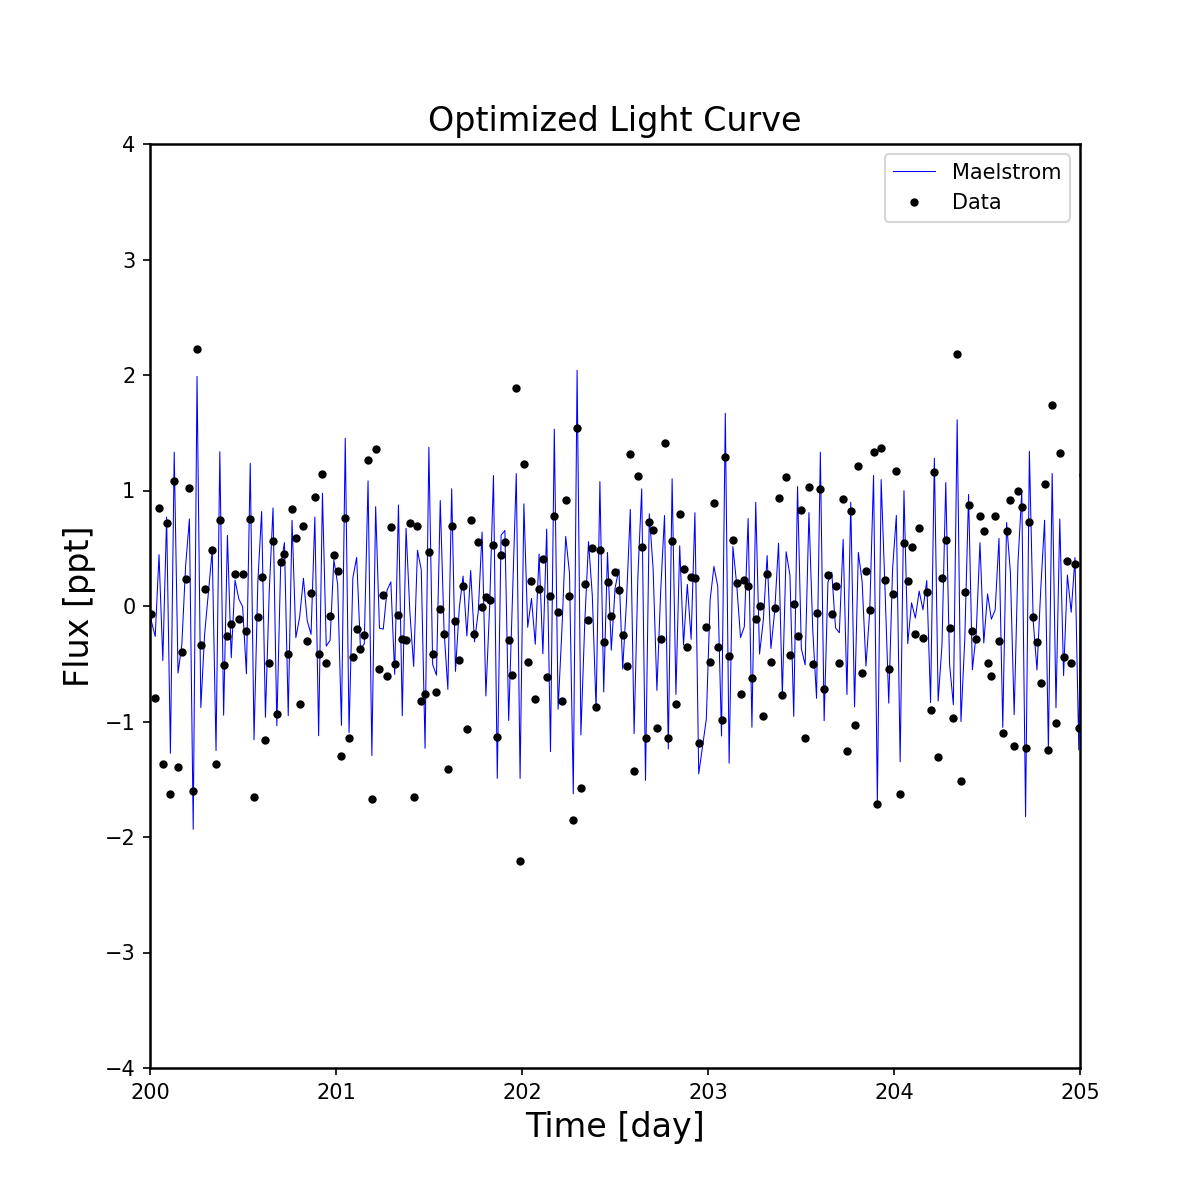
\includegraphics[width=1\linewidth]{lightcurve_opt.png}
      \caption{Need new caption}
      \label{fig:LightcurveOptimized}
\end{figure}

It is evident in Fig \ref{fig:LightcurveOptimized} that the original light curve data (black points) agrees really well with the theoretical fit obtained by forward modelling the light curve.
Although we can derive this from the time delay signal, this does not provide any further information than the previous light curve signal other than it shows a good correlation with the light curve meaning the model produces good output.

\section{Conclusion}
This project aimed to analyze the orbital properties of a binary star, using the \textit{Maelstrom} in particular. This projected looked at forward modelling the light curve data of a pulsating binary star in the NGC 6866 open cluster located in the constellation Cygnus to optimize its orbital parameters. It is clear from Fig \ref{fig:timedelay} that the correlation between the original data (black points) and the theoretical model (blue curve) that the orbital parameters have been optimized. From these optimized parameters it is possible to create a simplistic plot of the orbit for this binary star with an estimation of the barycenter for the binary system. Likewise, It is also possible to recreate the original light curve using the optimized parameters and the results in Fig \ref{fig:LightcurveOptimized} show great agreement between the original data (black points) and theoretical data (blue curve). In conclusion, this projected showed the power of using an open source software such as \textit{Maelstrom} to model stellar data and optimize the orbital parameters of such data in return producing results that correlate with what is expected.

\bibliography{bibliography}        

\end{document}